\documentclass[11pt]{article}

\usepackage[utf8]{inputenc}
\usepackage[T1]{fontenc}
\usepackage{amssymb}
\usepackage[a4paper, left=2cm, right=2cm, top=3.5cm, bottom=3.5cm]{geometry}
\usepackage[french]{babel}

% Paragraph spacing
\setlength{\parskip}{1em}

% Fancy headers
\usepackage{fancyhdr}

% Captions for subfigures
\usepackage{subcaption}

% Footnote inside a caption
\usepackage{fnpos}
\usepackage{ftnxtra}

% Maths
\usepackage{amsmath}

% Todo notes
\usepackage{todonotes}

% Table of contents for bibliography
\usepackage[nottoc]{tocbibind}

% Inline monospace font
\def\code#1{\texttt{#1}}

% Figures
\usepackage{graphicx}

% Draw figures
\usepackage{tikz}

% Tikz node rotation
\usetikzlibrary{positioning}

% Usage: \rotnode[options]{rotation}{text}
\newcommand\rotnode[3][]{%
    \node [#1, opacity=0.0] (tmp) {#3};
    \node [draw, rotate around={#2:(tmp.center)}] at (tmp) {#3};
}

% Clickable links
\usepackage{hyperref}

% Table of contents depth
\setcounter{tocdepth}{2}

% Inline code
\usepackage{listings}
\usepackage{color}

\title{Intervalle de confiance}

\author{Othmane AJDOR}
\date{2018-2019}

\begin{document}
\maketitle

\pagebreak

\tableofcontents

\pagebreak

\section{Intervalle de confiance}

\subsection{Sondage}
Comment modéliser les réponses obtenues lors d'un sondage?\\
Soit n= nombre de sondés à 2 choix -> généralisation

Pour la personne $n_{i}$, $X^{}_{i}$ = 1 ou 0 (p ou $1-p$)

Supposant les elections entre Le Pen et Macron, si le sondage est effectué après un rally de Macron et aux personnes qui étaient présentes, le sondage n'aura pas de sens.

On fait l'hypothese que ce qu'une personne pense est different de ce pense une autre. De ce fait, elles sont indépendantes.

Le résultat obtenu après le sondage peut êtremodelisé par $\textbf{X} = \sum_{i=1}^{n} X_{i}$ où X represente le nombre de $X_{i}$ à 1 sur les n.\\
Cette variable aléatoire suit une loi binomiale $B(n;p)$.\\
Soit $n=1000$ et $X=600$, alors on estime p à l'aide de:\\

$E(X) = np$\\
    $E(X_{i}) = np$\\
    $E(X_{i}) \approx \frac{1}{n}\sum_{i=1}^{n}x_{i}$, $x_{i}$ sont les valeurs des $X_{i}$.\\
    $P_{est} = \frac{1}{n}\sum_{i=1}^{n}x_{i}$

\subsection{definition}
On appelle intervalle de confiance de seuil $\alpha$ pour un parametre $\theta$ inconnu un intervalle I dont au moins une des bornes est une variable aleatoire reelle telle que :
$P(\theta \in I) = 1 - \alpha$.

Plus le seuil est faible, plus l'intervalle est grand.\\
On prend souvent $\alpha$ à 5\% ou alors 1\% pour les risques sanitaires où on veut limiter les risques.\\

\
\subsubsection{Exemple : IC pour la moyenne d'une loi normale}
Soit $n=20$  $\bar{x_{n}}=64$  $s_{n}=5=\frac{1}{n}\sum_{i=1}^{n}x_{i}$.

IC est obtenu à l'aide d'une fonction pivotale.
C'est une VA qui depend des choses qui nous interessent, ici n mais dont on connait parfaitement les lois. Elle nous permet de faire des calculs de probabilités.\\

Si les $X_{i}$ $N(m,\sigma^{2})$ et sont independantes, alors $Z=\sqrt{(n-1)}\frac{\bar{X_{n}}}{S_{n}}$  suit une loi de Student(n-1).

\centerline{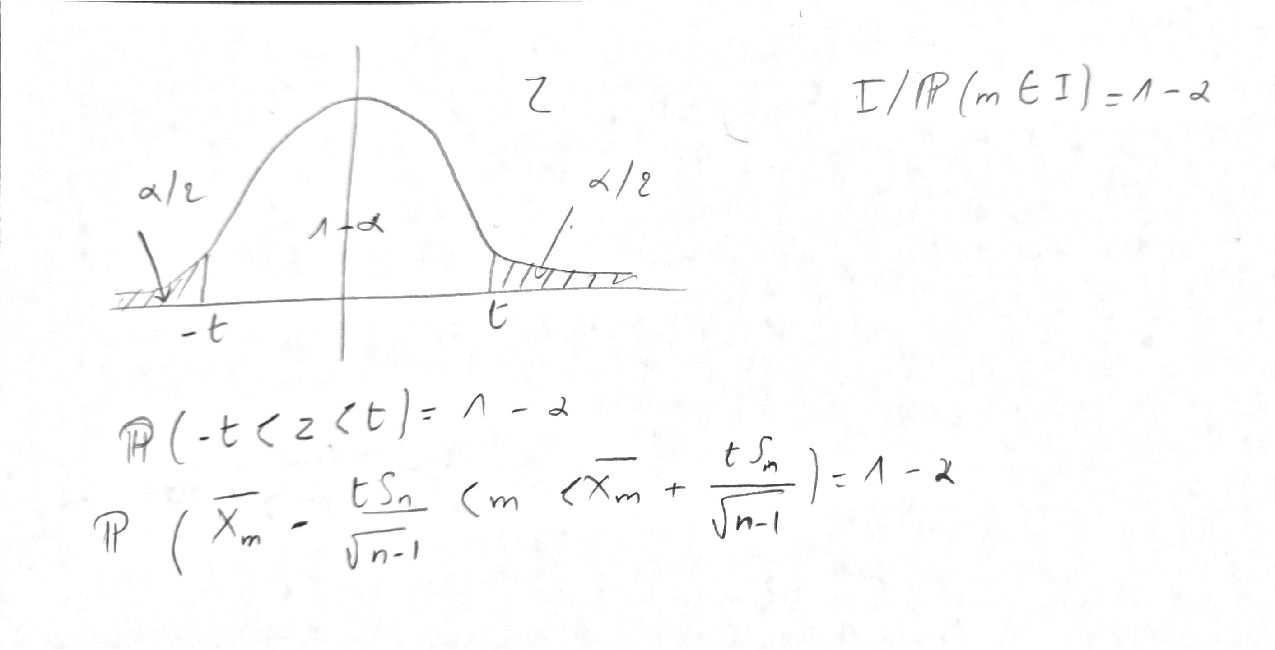
\includegraphics[scale=0.6]{img/ic.pdf}}

Soit $n=20$,  $\bar{x_{n}}=64$,  $s_{n}=5$, $t_{5\%} = 2.1$, $t_{5\%} =2.9$ 

\centerline{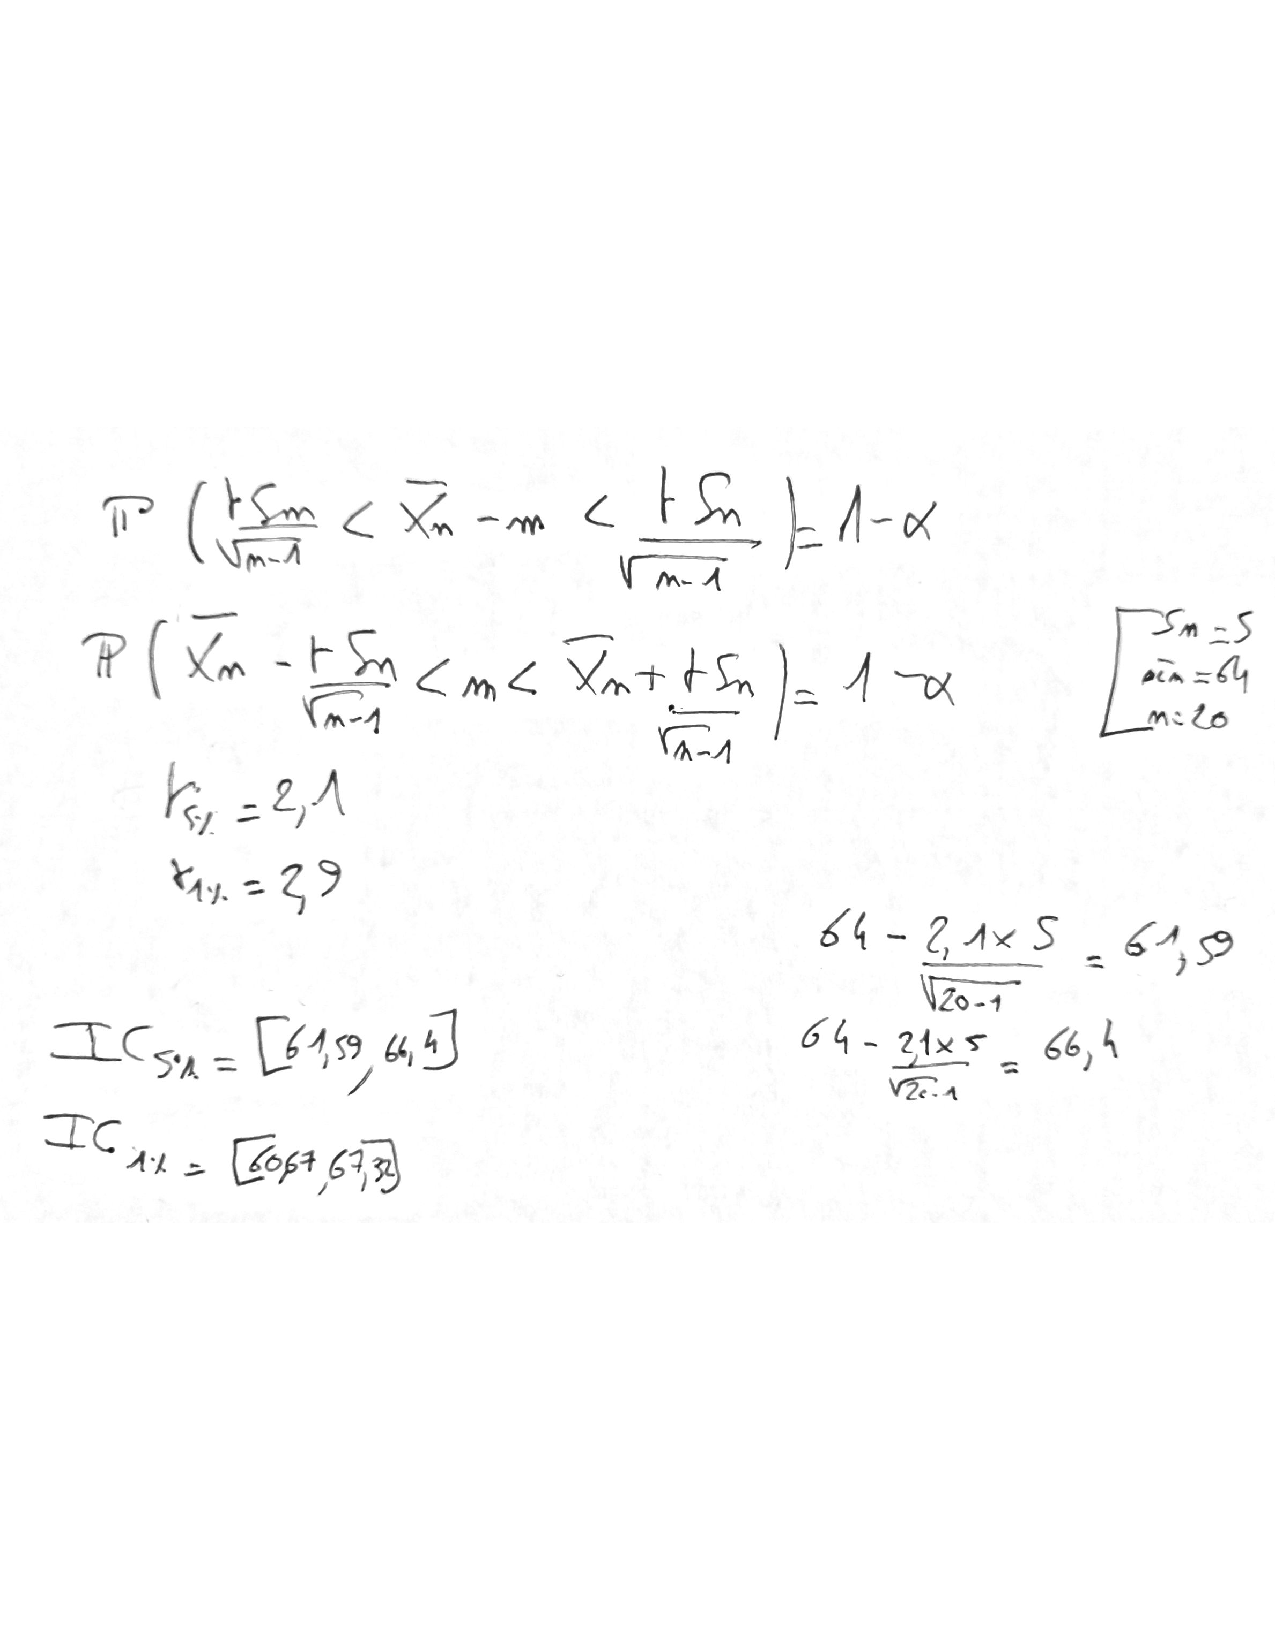
\includegraphics[scale=0.6]{img/calcul_ic.pdf}}

$IC_{1\%} = [60.7, 67.3]$ \qquad
$IC_{5\%} = [61, 66]$

\end{document}